\documentclass{mpaper}

\usepackage{graphicx}
\usepackage[numbers,sort&compress]{natbib}
\usepackage{amsmath}

\begin{document}

\title{Statistical Model Updates in Distributed Computing:\\ An Optimal Stopping Theory Perspective}
\author{Ekaterina Aleksandrova}
\matricnum{2133352a}

\maketitle

\begin{abstract}
This paper explores a decision technique of when to update statistical learning models in Intelligent Edge Devices given the underlying change in the context distribution. The model update scheduling takes into consideration the optimal time for minimizing the network overhead while preserving the prediction accuracy of the models. The paper presents a comparison between a proposed model updating approach and 4 other update delaying policies, an evaluation of the performances and a discussion on the strengths and weaknesses of the proposed policy.
\end{abstract}

\section{Introduction}

The Internet of Thing (IoT) environments have been gaining popularity since the end of the 20th century, transforming small environments into large scale ecosystems, 
whose cores (cloud data centers) require massive computational 
power to process all the received data and a substantial network overhead in order to receive all the needed raw data.

However, as this has proven to be inefficient, a solution has been provided in the form of Edge Computing environments, which push most of the computations to the edge of the network (e.g. sensors, mobile devices, etc.) taking advantage of the computational capabilities of modern devices. They deliver the processed data to the cloud in the form of partially or entirely extracted knowledge \cite{anagnostop2014}.

This also contributes as a security measure, because raw data is processed locally on the sensing device. Moreover, it is a method for decreasing network traffic, as the sent model representations of the data have smaller size compared to the raw data.

The edge computing method significantly reduces the required computational power but the acquired knowledge still needs to be transferred to the cloud on each iteration with a considerable communication overhead and other complications explained further ahead in this paper. 

\subsection*{Statement of the problem}
The main problem which this project aims to resolve is formulating an optimal waiting time criteria based on made observations on multivariate contextual data. The algorithm will decide when a model representation of the sensed data is sent from an edge node to an edge gateway in order to minimise the communication overhead and preserve or increase the accuracy of the generated models.

% The formulation of the Model Update problem is as follows:\\
% $\bullet$ A hardware structure is given as follows a sensing node transmitting data to the gateway.\\
% $\bullet$ At each time $t=0,1,2,3,...$ a model is generated using a constant sliding window of size $w$ (contains multivariate contextual observations $X_{k},X_{k+1},...,X_{k+w}$).\\
% $\bullet$ For each model we can obtain the Mean Squared Error (MSE) value based on the fitted data currently available at time $t$ in the edge node.\\
% $\bullet$ At $t=0$, a model is generated over the first $w$ datapoints ($X_{0},X_{1},...,X_{w}$) and sent from the edge node to the edge gate.\\
% $\bullet$ If $t=\infty$, it would mean that stopping has not occurred and a model update is never sent to the edge gateway.\\
% $\bullet$ Once a new model is obtained the previous one is discarded, therefore, if the previous one has had higher accuracy, it is no longer available to be shared with the edge gateway.

\textbf{RQ: How can waiting time and model accuracy at the edge gateway be maximised while minimising the communication to the gateway and computational complexity at the sensing node level?}

\section{Background}
\subsection*{Knowledge sharing in IoT environments}
Given a sample path in an IoT system consisting of a sensing node, a local edge gateway and a central data node as en endpoint, the multihop transmission can increase energy consumption when the gateway is busy and the data has to be passed to the central node \cite{shi2016}. When data processing is not performed at the edge level, if $N$ multivariate datapoints are sensed and sent through the network, that results in $N$ number of transmissions. However, if the data is processed at the edge, the result is a linear model representation of the data ($y = \alpha\cdot X + \beta$), where only the parameters $\alpha, \beta$ are being passed through the network reducing the energy consumption \cite{tanluizhang2011}.\\
Due to Wireless Sensor Networks (WSNs) used in remote locations (e.g. rainforest sensors  \cite{rainforests2009}, surface and mine monitoring \cite{Akkas2018}, water pollution detectors\cite{waterwsn2017}, etc.) are usually being powered by a battery, therefore, the energy consumption of the sensing devices should be minimised as much as possible to reduce the amount of human interaction required to replace the exhausted batteries. Such interaction with the device may distort the environment and introduce incorrect data and if the sensors are placed at locations with difficult access that could increase the financial cost or even cause danger to the person responsible for the replacement.\\
Other similar sensor systems rely on renewable energy, most widely used is solar energy, which could be slower to harvest in environments such as rainforests \cite{rainforests2009}, therefore, having a power efficient device is a must in order to have a well-functional system.\\
Another concern with communicating processed data on every sensing iteration is that it is possible that the data contains bias (e.g. missing or corrupted datapoints) \cite{anagnostop2016} which then when passed to the gateway can potentially be used to make inaccurate predictions of the sensed environment.\\
A way of minimising the energy cost of an edge device even more is by reducing the number of the data transmissions. This could be performed by introducing a certain delay in the delivery of the up-to-date model \citep{anagnostop2014, anagnostop2016, anagnostopkolomvatos2016}, at the cost of allowing a reasonable error in the data. 
The approach is as follows, if a data model is generated at the edge node and sent to the edge gateway, on the next iteration, if the node does not detect a significant change between the initially modelled data and the currently sensed dataset, no communication is made between the edge node and the edge gateway.\\
Deciding when to send a new updated model to the edge gateway from the node before the accuracy has degraded beyond a reasonable threshold can be looked from a slightly different angle. 

\subsection*{Optimal knowledge communication}
According to Thomas Ferguson from UCLA \cite{UCLAbook}, the theory of optimal stopping is attempting to solve exactly the problem stated above - choosing a time to take a given action (in this case to stop and update the model at the edge gateway) based on sequentially observed random variables, hence, a known distribution, in order to maximise an expected reward or minimise an expected cost. \\
And based on that formulation, there are several variations of the problem whose solutions are used as a basis to problems in Computing Science. Two relevant examples are the so called \emph{House-Selling} problem and the \emph{Quickest Change Detection} problem. 

\textbf{A.} The House-Selling problem explores the attempt to stop and sell a house at the highest offer by taking into account a cost, such as living cost or real estate agency commission, for each rejected offer.\\
This problem relates to the approach that waiting can be penalised, the way Tian et al. use it in their "cost-aware" update policy algorithm \cite{tian18}. There it can be seen that the decision on whether to update an outdated model with the current one is based on how much it was lost (how big the "regret" is) since the update was not performed in the past with a better model at that time. And once a tolerance threshold is passed, an update is inevitable, which also prevents additional unneeded retraining computations. 

\textbf{B.} Another base problem is the Change Point Detection problem, which concerns the exploration of the context distribution, stopping when a change is detected but penalising when the algorithm has signalled a false alarm \cite{UCLAbook}. 
Two researchers have investigated two different approaches based on their initial assumptions on the distribution. 
On one hand, there is Shiryaev \cite{shiryaev1963} who provides an optimal solution to the problem using a Bayesian approach. 
And then there is the proposed non-Bayesian solution using the CuSum algorithm provided by Page \cite{page1954}, which was later proven to be optimal by Moustakides \cite{moustakides1986} based on the formulation of the problem by Lorden \cite{lorden1971}.

In a recent publication, Lau and Tay\cite{lautay2018} introduce the idea of having a "critical change" and a "nuisance change" in distributions, where the critical change is of highest importance and should be detected, as opposed to the nuisance change which should be ignored by the algorithm. They propose two different algorithms using a Bayesian and a non-Bayesian approach, which then are compared to the performance for both types of change against the naive 2-stage procedures by Page\cite{page1954} and Shiryaev\cite{shiryaev1963}.

For their non-Bayesian approach, the authors compare their proposed algorithm with the naive 2-stage CuSum. The naive approach uses two separate thresholds, $\beta_c$ for the critical change and $\beta_n$ for the nuisance change, on the cumulative sum of the log-likelihood ratio of the normal distribution and the distributions after the nuisance and the critical change in order to detect the critical changes.
According to the authors, their non-Bayesian procedure, which is based on the Generalised Likelihood Ratio test, performs more accurately than the naive 2-stage optimal CuSum algorithm.

\section{Methodology}

%explain rationale behind each policy [N, E, A, M, C, OST]
The main focus of this paper is to present and experiment with the optimal update postponing algorithm for reducing the communication rate but preserving the quality of the context. 
The minimal assumption behind the environment contains a sensor node and an edge gateway device. 

On the first iteration of the algorithm, the sensing node is responsible for gathering environmental data and generating a statistical or machine learning model from the first \textbf{\emph{w}} contextual observations. The model is then temporarily stored on the sensing device but also communicated with the edge gateway.

On each next iteration, a new observation is received and appended to the currently stored sensor dataset of size \textbf{\emph{w}} while the observation with the oldest timestamp is discarded. A new model is generated representing the updated dataset. By fitting the dataset on the old and the new model, two mean squared errors (MSE) can be obtained:

\textbf{[$e$]} from the model the edge gateway has previously received and

\textbf{[$e'$]} from the model based on the most up-to-date sensed data.

Given that the latest model of the sensor node satisfies a certain criteria, a decision is made to communicate the model to the edge gateway. This also requires that the temporarily stored outdated model at the sensing device is also updated to correctly represent the disseminated local knowledge in the system.

\subsection*{Optimal Postponing Policy}
The postponing policy is based on the CuSum algorithm \cite{page1954}, which detects a change in the distribution using the cumulative sum of the absolute error difference between the two MSEs:
\begin{align}
    Z_k &= \Delta e_k = | e'_k - e_k |\\
    S_n &= \Delta e_n + \Sigma_{k=0}^{n-1} \Delta e_k\\
    S_n &= Z_k + S_{n-1}\label{eq:1}
\end{align}

A threshold $\Theta$ is placed to determine the acceptable error sum and is used to determine if the algorithm should be penalised or rewarded with a penalty/reward value $V_t$.
\begin{equation}\label{reward}
    V_t = \Bigg\{ \begin{tabular}{c}
                  $t\ \text{if}\ S_t \leq \Theta$ \\
                  $-B\ \text{if}\ S_t > \Theta$
                  \end{tabular}
\end{equation}

Taking into consideration that the expected reward $E[V_t]$ must be a positive value, we can calculate the probability interval that the cumulative sum is less than or equal to the set threshold.
\begin{equation}
    P(S_t \leq \Theta) > \frac{B}{t+B}
\end{equation}

\emph{\textbf{Proof:}} \\
From the reward function in (\ref{reward}) we can derive the expected reward function $E[V_t]$. 
\begin{equation}
\begin{split}
    E[V_t] & = t * P(S_t \leq \Theta) + (-B * P(S_t > \Theta))\\
    & = t * P(S_t \leq \Theta) - B * (1 - P(S_t \leq \Theta))
\end{split}
\end{equation}

Given that we aim is to not exceed the specified threshold $\Theta$, then the result of the reward function has to always be a positive value $E[V_t] > 0$. From this we can derive the probability of the absolute error sum not exceeding the threshold.
\begin{multline*}
    E[V_t] = (t + B) * P(S_t \leq \Theta) - B > 0\\
    =>  P(S_t \leq \Theta) > \frac{B}{t+B}
\end{multline*}

\begin{align*}
    E[V_{t+1}|S_t\leq\Theta] = (t+1+B)*P(S_{t+1}\leq\Theta) - B
\end{align*}
However, it is known from Eq.(\ref{eq:1}) that:
\begin{equation*}
    S_{t+1} = Z_{t+1} + S_t
\end{equation*}

Therefore, 
\begin{equation*}
    P(S_t + Z \leq \Theta) = P(Z\leq\Theta-S_t)
\end{equation*}


\subsection{Compared Policies}

In order to evaluate the performance of the presented algorithm 4 other policies are implemented, which rely either on certain statistics of the data or on pure randomness:\\
Median policy, Random policy, Accuracy policy, CuSum policy \cite{cusum_pierre}.

\subsubsection{Median Policy}

The Median Policy has an initially learned median of the previously seen data calculated on the absolute error difference values given that the initial model is never updated. 
The rationale behind this is to explore the assumed worst case scenario of the error difference. This assumes that the closer the timestamps of two models are, the lower the error difference between them is and respectively, the further away the timestamps of two models are, the higher their error difference is.

Using a fraction $\alpha$ of the median value the policy determines whether the current absolute error difference is a tolerable amount or if it indicates that the newly sensed data is significantly outdated and needs to be communicated with the edge gateway.

This policy is expected to reduce communication by being more tolerant towards initial small abrupt changes and detecting continuously increasing values.

==TODO: place a pseudo code snippet==

\subsubsection{Random Policy}
The random policy is intended to be sending updates of the latest model to the edge gateway with the same probability as the OST policy.
The aim of the policy is to show that even if the number of updates is approximated to the optimal value, the accuracy of the models at the edge gateway would still suffer a decrease.

==TODO: place a pseudo code snippet==

\subsubsection{Accuracy Policy}
The accuracy policy works by comparing the MSE of the old model and the most up-to-date model and once a decrease in the accuracy is detected, the latest model is sent to the edge gateway.
The policy aims to present a naive algorithm for reducing communication but preserving accuracy as high as possible.

==TODO: place a pseudo code snippet==

\subsubsection{CuSum Policy}
The algorithm implemented here relies on the direct form of the CuSum algorithm explained by Granjon \cite{cusum_pierre}.

For the execution of the algorithm, two assumptions of the distributions are made representing the two hypothesis and the algorithm aims to decide which hypothesis represents the current sample of data. 
Firstly, the $\mathcal{H}_0$ no change hypothesis which refers to the "good distribution" is assumed to be the distribution of the absolute error difference when the edge gateway model is communicated on every iteration. On the contrary, the "bad distribution" represented by the changed distribution $\mathcal{H}_1$ is assumed to be the distribution of the absolute error difference when the model is communicated only on the first iteration and then never again.

Given the assumption that the absolute error differences $Z_0, Z_1, \dotsc , Z_n $ are continuous independent random variables. In this case a gamma distribution is a good choice to represent the data  [Fig.\ref{fig:goodvsbad}], relying on the two flexible parameters for scale and shape of the probability density function of the distribution.

\begin{figure}[h]
    \centering
    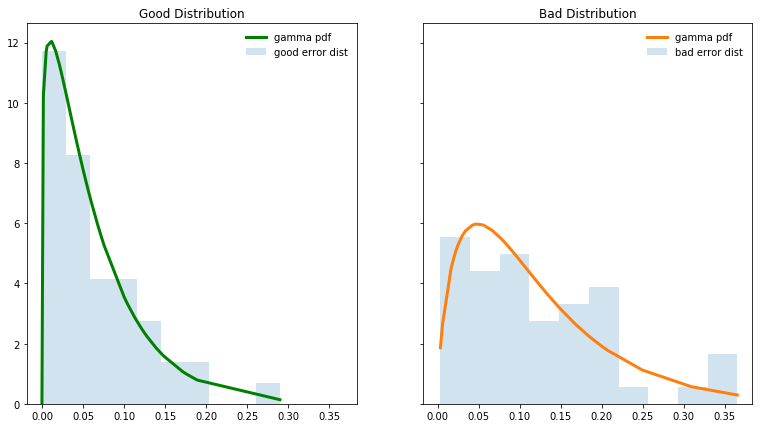
\includegraphics[scale=0.3]{imgs/goodVSbad.png}
    \caption{Gamma distribution approximation on GNFUV data using Linear Regression}
    \label{fig:goodvsbad}
\end{figure}

When a new absolute error difference is calculated it is then fitted in the two probability density function for each of the two distributions. The logarithmic ratio of the probability of the absolute error belonging to either the good or the bad distribution determines whether $\mathcal{H}_0$ or $\mathcal{H}_1$ is rejected.

==TODO: place a pseudo code snippet==

\section{Evaluation}

\subsection*{Data sets}
Two time-series datasets will be used in order to apply the proposed approach and perform the previously discussed experiments.
\\$\bullet$ \textbf{GNFUV Unmanned Surface Vehicles Sensor Data Data Set} \cite{harth2018} - a dataset produced by 4 Unmanned Surface Vehicle sensing devices which observed and recorded timestamped multivariate contextual environmental data using temperature and humidity sensors. The collected data will be associated with the Linear Regression task performed in the experiments for each policy. The generated linear regression models are aimed at predicting the environmental humidity based on the sensed temperature.
\\$\bullet$ \textbf{Gas sensors for home activity monitoring Data Set } \cite{HUERTA2016169} - a timestamped dataset containing readings from temperature, humidity and 8 metal-oxide(MOX) gas sensors of a contained environment where either or not a stimuli is presented. The collected data will be used in the Support Vector Regression(SVR) (with an RBF kernel) task in order to assess the 5 policies. The generated support vector models are aimed at predicting the level of MOX gas based on the vector of detected humidity and temperature.
\subsection{Experimentation}
% experiment set up for Lin Reg
% place plot of all policies abs error rate for lin reg
\begin{figure}[h]
    \centering
    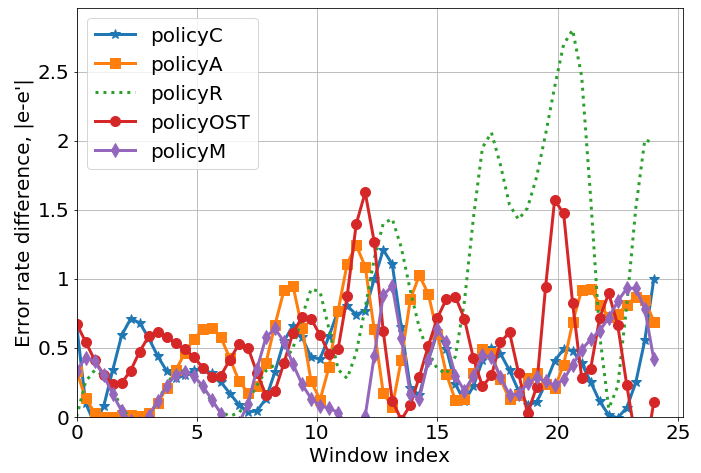
\includegraphics[scale=0.3]{imgs/lin_reg_pi3_w25.png}
    \caption{Absolute error difference for SUV sensor system, s=pi3, w=25, using Linear Regression}
    \label{fig:err_lin_reg_pi3}
\end{figure}

\begin{figure}[h]
    \centering
    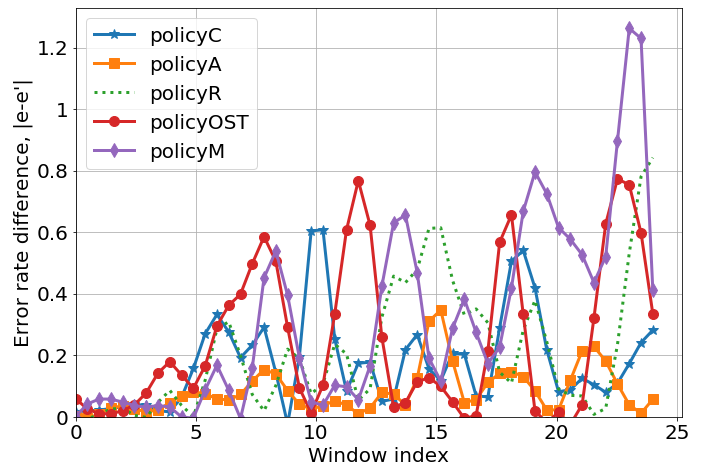
\includegraphics[scale=0.3]{imgs/lin_reg_pi4_w25.png}
    \caption{Absolute error difference for SUV sensor system, s=pi4, w=25, using Linear Regression}
    \label{fig:err_lin_reg_pi4}
\end{figure}
% talk about one-way anova results and tukey ttest on waiting time
% place plot
% talk about one way anova results and tukey ttest on abd error rate

% experiment set up for SVR
% place plot of all policies abs error rate for SVR
\begin{figure}[h]
    \centering
    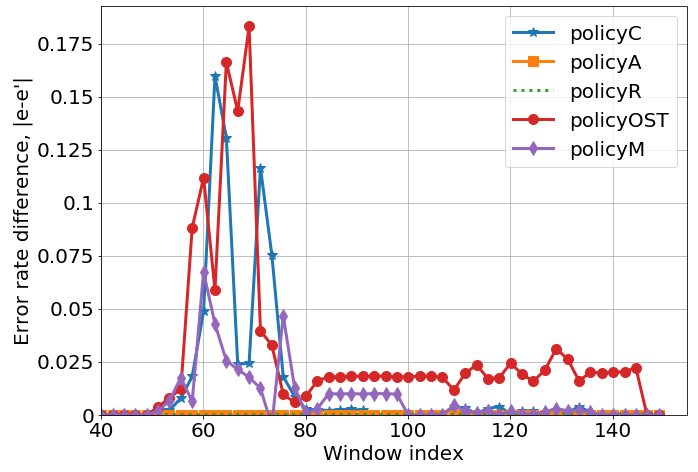
\includegraphics[scale=0.3]{imgs/svr_rbf_R3_w25.png}
    \caption{Absolute error difference for HT sensor system, s=R3, w=25,
    using Support Vector Regression with RBF Kernel 
    given an artificial change at 40th window iteration}
    \label{fig:err_rbf_svr_R3}
\end{figure}

\begin{figure}[h]
    \centering
    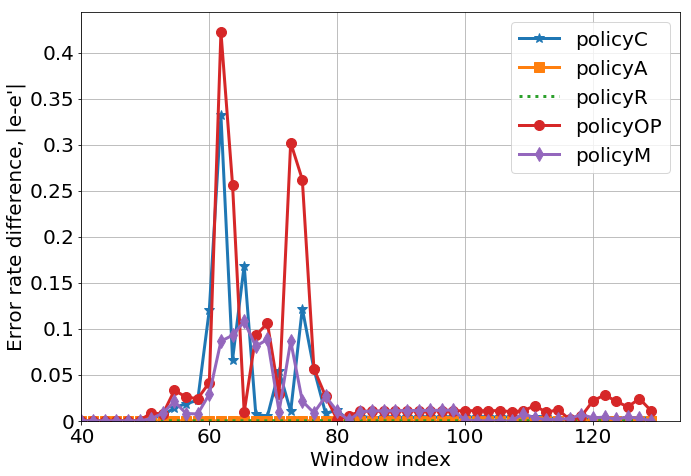
\includegraphics[scale=0.3]{imgs/svr_rbf_R5_w25.png}
    \caption{Absolute error difference for HT sensor system, s=R5, w=25,
    using Support Vector Regression with RBF Kernel 
    given an artificial change at 40th window iteration}
    \label{fig:err_rbf_svr_R5}
\end{figure}
% talk about one-way anova results and tukey ttest on waiting time
% place plot
% talk about one way anova results and tukey ttest on abd error rate

\subsection{Evaluation summary}
% place table with all policies and say when each is good for accurate models and when is good to wait and so on

\section{Conclusions}

\subsection*{Future work}

{\bf Acknowledgments.}
This is optional; it is a location for you to thank people

\bibliographystyle{abbrv}
\bibliography{example.bib}


\end{document}